
First, creat a package for your class.  Select the project you created in the package explorer, right click, and select
"New" -$>$ "Package" -$>$ "Other" from the context menu. You have to look for "Package" in the "Java" folder.\\\\
\begin{figure}[htbp]
	\centering
		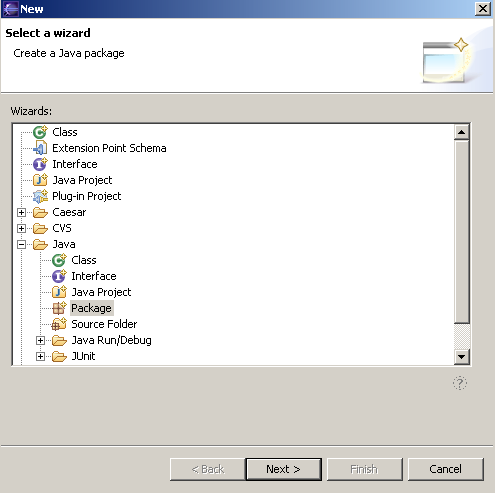
\includegraphics[width=0.70\textwidth]{images/package.png}
	\label{fig:package}
\end{figure}\\\\
Name the package "myPackage" then click finish.\\\\
Select the package you just created, and from the context menu select "New" -$>$ "Class". Name the
class "HelloWorld" and select the option to let Eclipse create a new main method for you. Click "Finish".\newpage
Edit the text in the editor so that it looks something like this:\\\\
\begin{center}
	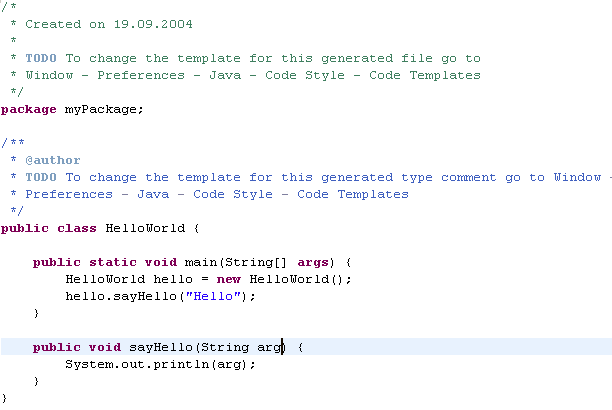
\includegraphics[width=0.80\textwidth]{images/code.png}
\end{center}
	
Save the file.\\\\

Notice that unlike in a Java project, there was no eager parsing of the buffer as you typed (the outline view didn't update). Your Eclipse workbench should be looking something like this:\\
\begin{center}
	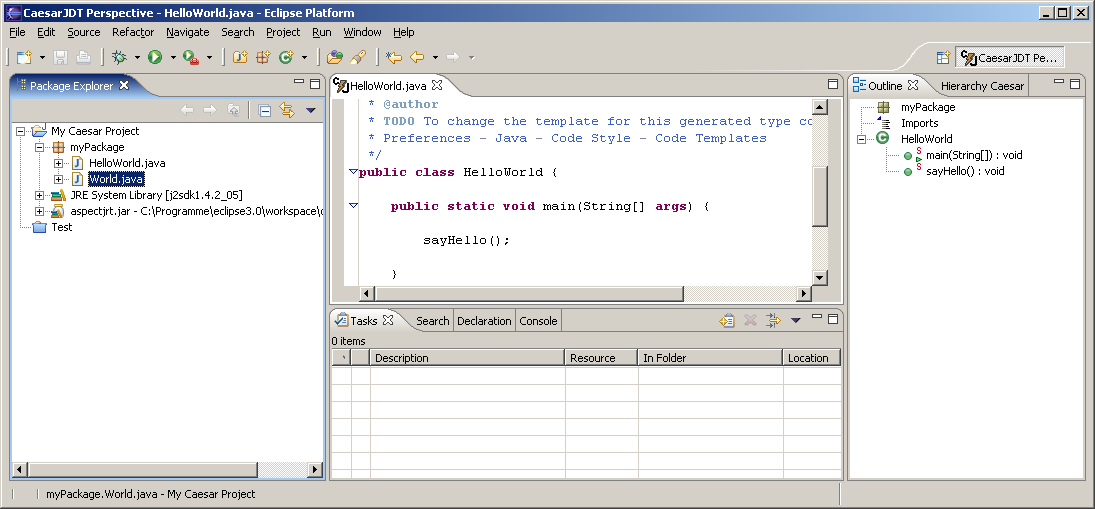
\includegraphics[width=1.0\textwidth]{images/workspace_newclass.png}
\end{center}